\documentclass{beamer}
\mode<presentation>
\usepackage{amsmath}
\usepackage{amssymb}
%\usepackage{advdate}
\usepackage{adjustbox}
\usepackage{subcaption}
\usepackage{enumitem}
\usepackage{multicol}
\usepackage{mathtools}
\usepackage{listings}
\usepackage{url}
\def\UrlBreaks{\do\/\do-}
\usetheme{Boadilla}
\usecolortheme{lily}
\setbeamertemplate{footline}
{
  \leavevmode%
  \hbox{%
  \begin{beamercolorbox}[wd=\paperwidth,ht=2.25ex,dp=1ex,right]{author in head/foot}%
    \insertframenumber{} / \inserttotalframenumber\hspace*{2ex} 
  \end{beamercolorbox}}%
  \vskip0pt%
}
\setbeamertemplate{navigation symbols}{}

\providecommand{\nCr}[2]{\,^{#1}C_{#2}} % nCr
\providecommand{\nPr}[2]{\,^{#1}P_{#2}} % nPr
\providecommand{\mbf}{\mathbf}
\providecommand{\pr}[1]{\ensuremath{\Pr\left(#1\right)}}
\providecommand{\qfunc}[1]{\ensuremath{Q\left(#1\right)}}
\providecommand{\sbrak}[1]{\ensuremath{{}\left[#1\right]}}
\providecommand{\lsbrak}[1]{\ensuremath{{}\left[#1\right.}}
\providecommand{\rsbrak}[1]{\ensuremath{{}\left.#1\right]}}
\providecommand{\brak}[1]{\ensuremath{\left(#1\right)}}
\providecommand{\lbrak}[1]{\ensuremath{\left(#1\right.}}
\providecommand{\rbrak}[1]{\ensuremath{\left.#1\right)}}
\providecommand{\cbrak}[1]{\ensuremath{\left\{#1\right\}}}
\providecommand{\lcbrak}[1]{\ensuremath{\left\{#1\right.}}
\providecommand{\rcbrak}[1]{\ensuremath{\left.#1\right\}}}
\theoremstyle{remark}
\newtheorem{rem}{Remark}
\newcommand{\sgn}{\mathop{\mathrm{sgn}}}
\providecommand{\abs}[1]{\left\vert#1\right\vert}
\providecommand{\res}[1]{\Res\displaylimits_{#1}} 
\providecommand{\norm}[1]{\lVert#1\rVert}
\providecommand{\mtx}[1]{\mathbf{#1}}
\providecommand{\mean}[1]{E\left[ #1 \right]}
\providecommand{\fourier}{\overset{\mathcal{F}}{ \rightleftharpoons}}
%\providecommand{\hilbert}{\overset{\mathcal{H}}{ \rightleftharpoons}}
\providecommand{\system}{\overset{\mathcal{H}}{ \longleftrightarrow}}
	%\newcommand{\solution}[2]{\textbf{Solution:}{#1}}
%\newcommand{\solution}{\noindent \textbf{Solution: }}
\providecommand{\dec}[2]{\ensuremath{\overset{#1}{\underset{#2}{\gtrless}}}}
\newcommand{\myvec}[1]{\ensuremath{\begin{pmatrix}#1\end{pmatrix}}}
\let\vec\mathbf

\lstset{
%language=C,
frame=single, 
breaklines=true,
columns=fullflexible
}

\numberwithin{equation}{section}

\title{4.7.54}
\author{Rushil Shanmukha Srinivas \\EE25BTECH11057 \\ Electrical Enggineering ,\\IIT Hyderabad.}

\date{\today} 
\begin{document} 

\begin{frame}
\titlepage
\end{frame}

\section*{Outline}
\begin{frame}
\tableofcontents
\end{frame}
\section{Problem}
\begin{frame}
\frametitle{Problem Statement}
\textbf{Question} : Find the vector equations of the line passing through the point (1,2,-4) and  perpendicular to the two lines 

$\frac{x-8}{3} = \frac{y+19}{-16} = \frac{z-10}{7}$ and
$\frac{x-15}{3} = \frac{y-29}{8} = \frac{z-5}{-5}$.
\end{frame}
\section{Solution}
\subsection{Equation of Line in Vector form}
\begin{frame}
\frametitle{Equation of Line in Vector form}
%\framesubtitle{Literature}
\textbf{Solution} :
 Given the line passes through the point
\begin{align}
\vec{A} = \myvec{1\\2\\-4}
\end{align}
The line is also perpendicular to
\begin{align}
\frac{x-8}{3} = \frac{y+19}{-16} = \frac{z-10}{7} ,
\frac{x-15}{3} = \frac{y-29}{8} = \frac{z-5}{-5}.
\end{align}
The direction vector of the line is given by
\begin{align}
\myvec{
3 & -16 & 7 \\
3 & 8 & -5} \vec{m} = 0 \xleftrightarrow{R_2\longrightarrow R_2-R_1}
\myvec{
3 & -16 & 7 \\
0 & 24 & -12}
\end{align}
\begin{align}
\myvec{
3 & -16 & 7 \\
0 & 24 & -12} \xleftrightarrow{R_1\longrightarrow 3R_1+2R_2}
\myvec{
9 & 0 & -3 \\
0 & 24 & -12}
\end{align}
\begin{align}
\myvec{
9 & 0 & -3 \\
0 & 24 & -12} \xleftrightarrow{R_1\longrightarrow \frac{R_1}{9}}
\myvec{
1 & 0 & \frac{-1}{3} \\
0 & 24 & -12}
\end{align}
\end{frame}
\begin{frame}
\begin{align}
\myvec{
1 & 0 & \frac{-1}{3} \\
0 & 24 & -12} \xleftrightarrow{R_2\longrightarrow \frac{R_2}{24}}
\myvec{
1 & 0 & \frac{-1}{3} \\
0 & 1 & \frac{-1}{2}} 
\end{align}
So \begin{align}
\vec{m}=\myvec{2\\3\\6} = Direction \ vector \ of \ line
\end{align}
The vector equation of the line is
\begin{align}
\vec{L_1} = \vec{A}+k\vec{m} = \myvec{1\\2\\-4}+k\myvec{2\\3\\6}
\end{align}

\end{frame}
\subsection{Plots}
\begin{frame}
\frametitle{Plots}
\begin{figure}
\centering
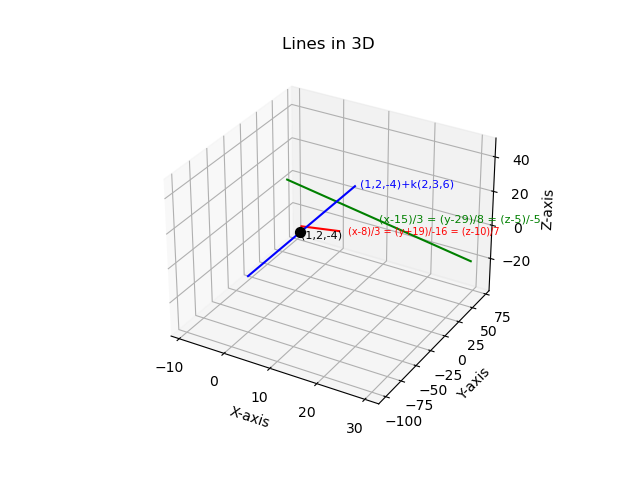
\includegraphics[width=0.9\columnwidth]{figs/fig7.png}
\caption{fig : Representation of Lines and Point}
\label{Fig7}
\end{figure}
\end{frame}
\section{C Code}
\begin{frame}[fragile]
\frametitle{C Code }
\begin{lstlisting}[language=C]
 #include <stdio.h>
// Function to compute cross product of two 3D vectors
void cross_product(double a[3], double b[3], double result[3]) {
    result[0] = a[1]*b[2] - a[2]*b[1];
    result[1] = a[2]*b[0] - a[0]*b[2];
    result[2] = a[0]*b[1] - a[1]*b[0];}

// Function to compute line equation point for given t
void line_equation(double t, double *x, double *y, double *z) {
    // Given point (1,2,-4)
    double p[3] = {1, 2, -4};
    // Given direction vectors of the two lines
    double d1[3] = {3, -16, 7};
    double d2[3] = {3, 8, -5};

    // Direction of required line = cross product of d1 and d2
    double d[3];
\end{lstlisting}
\end{frame}
\begin{frame}[fragile]
\begin{lstlisting}
    cross_product(d1, d2, d);
    // Simplify direction vector by dividing by GCD factor if desired
    // For this case, (24,36,72) → (2,3,6)
    d[0] = 2; d[1] = 3; d[2] = 6;

    // Parametric equation
    *x = p[0] + d[0]*t;
    *y = p[1] + d[1]*t;
    *z = p[2] + d[2]*t;}

// Convenience function for printing
void print_line(double t) {
    double x, y, z;
    line_equation(t, &x, &y, &z);
    printf("For t=%.2f -> (x, y, z) = (%.2f, %.2f, %.2f)\n", t, x, y, z);
}
\end{lstlisting}
\end{frame}
\begin{frame}[fragile]
\begin{lstlisting}
// Main function (for standalone execution)
int main() {
    printf("Line passing through (1,2,-4) and perpendicular to given lines:\n");
    printf("Vector form: r(t) = (1,2,-4) + t(2,3,6)\n\n");

    // Print some sample points
    for (int i = 0; i <= 5; i++) {
        print_line((double)i);
    }
    return 0;
}

\end{lstlisting}
\end{frame}

\section{Python Code}
\begin{frame}[fragile]
\frametitle{Python : call\_c.py}
\begin{lstlisting}
import ctypes
# Load the shared library compiled from line.c
# Make sure libline.so is in the same folder
lib = ctypes.CDLL("./libline.so")
# Setup the function signatures
# void line_equation(double t, double *x, double *y, double *z)
lib.line_equation.argtypes = [
    ctypes.c_double,
    ctypes.POINTER(ctypes.c_double),
    ctypes.POINTER(ctypes.c_double),
    ctypes.POINTER(ctypes.c_double)]
lib.line_equation.restype = None

# void print_line(double t)
lib.print_line.argtypes = [ctypes.c_double]
lib.print_line.restype = None
\end{lstlisting}
\end{frame}
\begin{frame}[fragile]
\begin{lstlisting}
# Example usage of the functions
if __name__ == "__main__":
    # Use line_equation() to get coordinates back into Python
    t = 2.0
    x = ctypes.c_double()
    y = ctypes.c_double()
    z = ctypes.c_double()
    lib.line_equation(t, ctypes.byref(x), ctypes.byref(y), ctypes.byref(z))
    print(f"Using line_equation from C: t={t} -> (x, y, z) = ({x.value}, {y.value}, {z.value})")

    # Use print_line() to let C handle printing
    print("\nCalling print_line from C:")
    lib.print_line(3.0)
    # Generate multiple points
    print("\nGenerating multiple points using print_line:")
    for i in range(6):
        lib.print_line(float(i))
\end{lstlisting}
\end{frame}

\begin{frame}[fragile]
\frametitle{Python Code for Plotting}
\begin{lstlisting}[language=Python]
import numpy as np
import matplotlib.pyplot as plt
from mpl_toolkits.mplot3d import Axes3D
# Given lines direction vectors
d1 = np.array([3, -16, 7])
d2 = np.array([3, 8, -5])
p1 = np.array([8, -19, 10])   # point on line 1
p2 = np.array([15, 29, 5])    # point on line 2
# New line
p0 = np.array([1, 2, -4])
d = np.array([2, 3, 6])
# Parameter ranges
t = np.linspace(-5, 5, 100)

# Line equations
line1 = p1[:, None] + d1[:, None]*t
line2 = p2[:, None] + d2[:, None]*t
\end{lstlisting}
\end{frame}
\begin{frame}[fragile]
\begin{lstlisting}
line3 = p0[:, None] + d[:, None]*t
# Plotting
fig = plt.figure()
ax = fig.add_subplot(111, projection='3d')
ax.plot(line1[0], line1[1], line1[2], color='r')
ax.plot(line2[0], line2[1], line2[2], color='g')
ax.plot(line3[0], line3[1], line3[2], color='b')

# Mark the point (1,2,-4)
ax.scatter(p0[0], p0[1], p0[2], color='k', s=50)
ax.text(p0[0], p0[1], p0[2]-4, "(1,2,-4)", color='k', fontsize=8)  # below the point
# Labels beside the lines
# Red line label -> shifted outward in x, but moved a bit downward
ax.text(line1[0][-1]+2, line1[1][-1]-2, line1[2][-1],
        "(x-8)/3 = (y+19)/-16 = (z-10)/7", color='r', fontsize=7)
# Green line label -> shifted upward compared to last version
mid_idx = len(t)//2
\end{lstlisting}
\end{frame}
\begin{frame}[fragile]
\begin{lstlisting}
ax.text(line2[0][mid_idx], line2[1][mid_idx]-3, line2[2][mid_idx],
        "(x-15)/3 = (y-29)/8 = (z-5)/-5", color='g', fontsize=8)

# Blue line label
ax.text(line3[0][-1]+1, line3[1][-1], line3[2][-1],
        "(1,2,-4)+k(2,3,6)", color='b', fontsize=8)
# Formatting
ax.set_xlabel("X-axis")
ax.set_ylabel("Y-axis")
ax.set_zlabel("Z-axis")
ax.set_title("Lines in 3D")

plt.savefig("../figs/fig7.png")
plt.show()

\end{lstlisting}
\end{frame}

\end{document}
  